\documentclass[11pt,a4paper]{article}
\usepackage[margin=1in]{geometry}
\usepackage[T1]{fontenc}
\usepackage[utf8]{inputenc}
\usepackage{lmodern}
\usepackage{hyperref}
\usepackage{enumitem}
\usepackage{xurl}
\usepackage{tikz}
\usepackage{float}
\usetikzlibrary{arrows.meta, positioning, shapes.geometric}
\hypersetup{colorlinks=true,linkcolor=blue,urlcolor=blue}
\newcommand{\codepath}[1]{\path{#1}}
\tikzset{
  box/.style={rectangle,draw,rounded corners,align=center,inner sep=3pt,minimum width=44mm},
  decision/.style={diamond,draw,aspect=2.2,align=center,inner sep=2pt},
  line/.style={-Latex}
}

\title{Phase-2 Deliverable: Dataset Governance}
\author{SIT Engine Documentation}
\date{\today}

\begin{document}
\maketitle

\section{Technical Description}
Dataset governance ensures baseline trace and residency assets evolve under controlled versioning, provenance updates, and deterministic validation gates.

\section{Implementation Fulfillment}
Governed assets live under \codepath{Phase-2/datasets/}; checks are executed through replay and determinism scripts in \codepath{Phase-2/tests/}.

\section{Design \& Architecture}
\subsection*{Function Attributes}
\begin{itemize}[leftmargin=*]
  \item \texttt{run\_golden\_suite.main()}: Inputs=manifest + replay inputs; Outputs=replayed outputs + pass/fail; Side effects=verifies dataset usability in engine replay; Failure modes=replay/invariant failure.
  \item \texttt{check\_determinism.main()}: Inputs=target list + manifests; Outputs=determinism pass/fail; Side effects=guarantees baseline reproducibility; Failure modes=hash mismatches.
  \item \texttt{sha256\_file()}: Inputs=artifact path; Outputs=SHA256 digest; Side effects=tracks immutable content identity; Failure modes=missing/corrupt file.
  \item \texttt{build\_manifest()}: Inputs=trace + mask paths + metadata; Outputs=manifest JSON; Side effects=pins dataset version and replay inputs; Failure modes=incomplete metadata.
\end{itemize}
\subsection*{Function Execution Details}
\begin{enumerate}[leftmargin=*]
  \item \texttt{run\_golden\_suite.main()}
  \begin{itemize}[leftmargin=*]
    \item Input attributes: manifest + replay inputs.
    \item Processing flow: verifies dataset usability in engine replay.
    \item Output attributes: replayed outputs + pass/fail.
    \item Failure behavior: replay/invariant failure.
  \end{itemize}
  \item \texttt{check\_determinism.main()}
  \begin{itemize}[leftmargin=*]
    \item Input attributes: target list + manifests.
    \item Processing flow: guarantees baseline reproducibility.
    \item Output attributes: determinism pass/fail.
    \item Failure behavior: hash mismatches.
  \end{itemize}
  \item \texttt{sha256\_file()}
  \begin{itemize}[leftmargin=*]
    \item Input attributes: artifact path.
    \item Processing flow: tracks immutable content identity.
    \item Output attributes: SHA256 digest.
    \item Failure behavior: missing/corrupt file.
  \end{itemize}
  \item \texttt{build\_manifest()}
  \begin{itemize}[leftmargin=*]
    \item Input attributes: trace + mask paths + metadata.
    \item Processing flow: pins dataset version and replay inputs.
    \item Output attributes: manifest JSON.
    \item Failure behavior: incomplete metadata.
  \end{itemize}
\end{enumerate}


\subsection*{Diagram A: End-to-End Design Flow}
\begin{figure}[H]
\centering
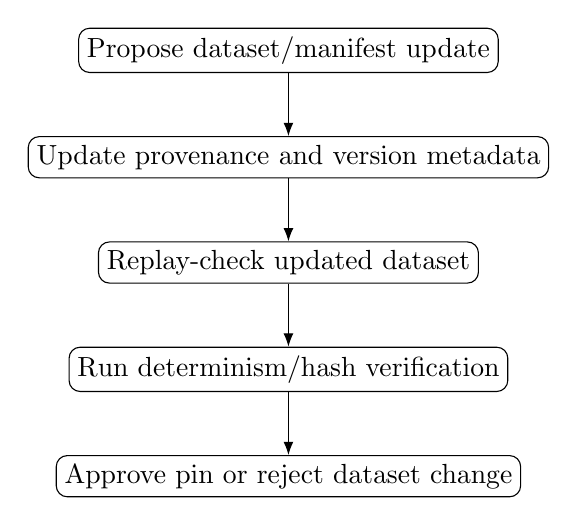
\begin{tikzpicture}[node distance=8mm and 12mm]
\node[box] (a) {Propose dataset/manifest update};
\node[box, below=of a] (b) {Update provenance and version metadata};
\node[box, below=of b] (c) {Replay-check updated dataset};
\node[box, below=of c] (d) {Run determinism/hash verification};
\node[box, below=of d] (e) {Approve pin or reject dataset change};
\draw[line] (a) -- (b);
\draw[line] (b) -- (c);
\draw[line] (c) -- (d);
\draw[line] (d) -- (e);
\end{tikzpicture}
\caption{Deliverable 08: End-to-End Design Flow}
\end{figure}

\subsection*{Diagram B: Function Interaction and Attribute Flow}
\begin{figure}[H]
\centering
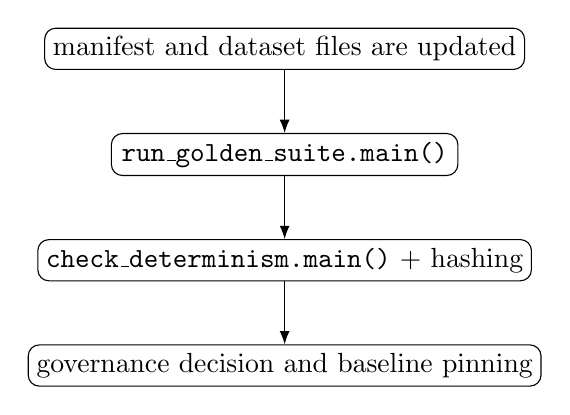
\begin{tikzpicture}[node distance=8mm and 12mm]
\node[box] (fa) {manifest and dataset files are updated};
\node[box, below=of fa] (fb) {\texttt{run\_golden\_suite.main()}};
\node[box, below=of fb] (fc) {\texttt{check\_determinism.main()} + hashing};
\node[box, below=of fc] (fd) {governance decision and baseline pinning};
\draw[line] (fa) -- (fb);
\draw[line] (fb) -- (fc);
\draw[line] (fc) -- (fd);
\end{tikzpicture}
\caption{Deliverable 08: Function Interaction and Attribute Flow}
\end{figure}

\end{document}
